\begin{frame}{Agent Capabilities and Safety}
    \framesubtitle{Tools}

    \begin{columns}[T,onlytextwidth]
        \begin{column}{0.55\textwidth}
            \textbf{LangChain tools available to the agent}
            \begin{itemize}
                \item[\faNetworkWired] \texttt{host\_configuration} \scriptsize situational awareness (interfaces, target/mgmt)
                \item[\faTerminal] \texttt{cli\_tool} \scriptsize arbitrary shell -- nmap, tshark, \ldots
                \item[\faCogs] \textbf{Drills as tools} \scriptsize \texttt{discover\_hosts}, \texttt{port\_scan} auto-wrapped
                \item[\faEnvelope] \texttt{send\_email} \scriptsize reports to a fixed recipient
                \item[\faUser] \texttt{human\_interaction\_hook} \scriptsize pause \& ask the operator
                \item[\faPlug] \textbf{MCP} \scriptsize external draw.io diagram server
            \end{itemize}
        \end{column}
    \end{columns}
\end{frame}


\begin{frame}{Implemented Scenarios}
    \framesubtitle{One static baseline, three AI scenarios}

    \begin{columns}[T,onlytextwidth]
        \begin{column}{0.5\textwidth}
            \uncover<1-> {
                \textbf{\faClipboardCheck~~Static Reference (baseline)}
                \begin{itemize}
                    \item \scriptsize Fixed drill chain: \texttt{arp-scan} $\rightarrow$ \texttt{nmap -sV} $\rightarrow$ NSE scripts
                    \item \scriptsize Deterministic, structured result, predictable errors
                \end{itemize}
            }

            \vspace{0.6em}
            \uncover<2-> {
                \textbf{\faRobot~~AI Agent}
                \begin{itemize}
                    \item \scriptsize single and multi-agent
                    \item \scriptsize unstructured and structured output
                    \item \scriptsize interactive with human interaction hook.
                    \item \scriptsize model independent
                \end{itemize}
            }
        \end{column}

        \begin{column}{0.5\textwidth}
            \uncover<3-> {
                \textbf{\faSearch~~AI Reconnaissance \scriptsize (main)}
                \begin{itemize}
                    \item \scriptsize 5-step prompt; \textbf{agent} picks nmap flags \& interprets results
                    \item \scriptsize Reports findings + vulnerability indicators
                \end{itemize}
            }
        \end{column}
    \end{columns}
\end{frame}


\begin{frame}{How We Integrated the LLM}
    \framesubtitle{NSAK as the harness -- the agent only reasons, the framework acts}

    \begin{columns}[T,onlytextwidth]
        \begin{column}{0.5\textwidth}
            \begin{itemize}
                \item[\faCogs] \textbf{Capabilities become tools} \scriptsize each drill is exposed to the agent
                \item[\faPlug] \textbf{Provider-agnostic} \scriptsize local (Ollama) and hosted models behind one interface, swapped via config
                \item[\faLayerGroup] \textbf{Cross-cutting middleware} \scriptsize one place to add logging, safety and context control around \emph{every} agent
            \end{itemize}
        \end{column}

        \begin{column}{0.5\textwidth}
            \onslide<4->{
                \begin{block}{One abstraction, three modes}
                    \scriptsize
                    The same agent powers \textbf{single-agent}, \textbf{multi-agent} and \textbf{interactive} scenarios.
                    \vspace{0.3em}\\
                    The remaining slides show the three concepts we had to solve to make this reliable.
                \end{block}
            }
        \end{column}
    \end{columns}
\end{frame}


\begin{frame}{Concept 1: Taming the Context}
    \framesubtitle{From one overloaded agent to a focused pipeline}

    \begin{columns}[T,onlytextwidth]
        \begin{column}{0.5\textwidth}
            \onslide<1-> {
                \textbf{\faExclamationTriangle~~The problem}
                \begin{itemize}
                    \item \scriptsize One agent does everything in a single long conversation
                    \item \scriptsize Every scan output piles up $\rightarrow$ the \textbf{context keeps growing}
                    \item \scriptsize Smaller models lose the thread and start failing
                    \item \scriptsize Cost and runtime become hard to predict
                \end{itemize}
            }
        \end{column}

        \begin{column}{0.5\textwidth}
            \onslide<2->{
                \textbf{\faProjectDiagram~~Our solution}
                \begin{itemize}
                    \item \scriptsize Split the task into \textbf{discovery $\rightarrow$ enumeration $\rightarrow$ assessment}
                    \item \scriptsize Each phase is a \textbf{fresh agent} with its own, small context
                    \item \scriptsize We pass on only the \textbf{distilled result}, not the whole history
                \end{itemize}
            }
        \end{column}
    \end{columns}

    \onslide<3->{
        \vspace{0.4em}
        \footnotesize \faInfoCircle~~Trade-off: rescues small models, but adds orchestration overhead that frontier models don't need.
    }
\end{frame}


\begin{frame}{Concept 2: Keeping the Operator in Control}
    \framesubtitle{The agent proposes -- the human decides on risky actions}

    \begin{columns}[T,onlytextwidth]
        \begin{column}{0.5\textwidth}
            \textbf{\faExclamationTriangle~~The problem}
            \begin{itemize}
                    \item \scriptsize An autonomous agent can run \textbf{any} command or send reports on its own
                    \item \scriptsize In a security context that is unacceptable without oversight
            \end{itemize}
        \end{column}

        \begin{column}{0.5\textwidth}
            \onslide<3->{
                \textbf{\faHandPaper~~Our solution}
                \begin{itemize}
                    \item \scriptsize The agent \textbf{pauses} before sensitive actions and asks for a decision
                    \item[\faTerminal] \scriptsize Shell commands $\rightarrow$ \textbf{approve} before they run
                    \item[\faEnvelope] \scriptsize Sending a report $\rightarrow$ \textbf{approve / reject}
                    \item[\faComments] \scriptsize Open questions $\rightarrow$ operator \textbf{responds} in free text
                \end{itemize}
            }
        \end{column}
    \end{columns}

    \onslide<4->{
        \vspace{0.4em}
        \footnotesize \faRedo~~After the decision the agent resumes exactly where it stopped -- no restart, no lost progress.
    }
\end{frame}
%
%\begin{frame}{Single- vs.\ Multi-Agent}
%    \framesubtitle{Addressing context size for smaller models}
%
%    \begin{columns}[T,onlytextwidth]
%        \begin{column}{0.5\textwidth}
\begin{frame}{Answering the Research Questions}
    \footnotesize

    \begin{itemize}
        \item[\textbf{RQ1}] \textbf{AI vs.\ static:} Same discovery power as baseline, no gains in speed/determinism.
        Adds value via \textbf{interpretation} (credentials, banner reasoning, severity scoring).

        \vspace{0.2em}
        \item[\textbf{RQ2}] \textbf{Operator support:} Converts scans into structured, severity-ranked output + next steps.
        \texttt{--interactive} preserves human control.

        \vspace{0.2em}
        \item[\textbf{RQ3}] \textbf{Deployment:} Scales to $\sim$35 hosts, highlights key risks.
        \textbf{Requires supervision} (reliability limits).
    \end{itemize}

\end{frame}%                \textbf{Single Agent}
%                \begin{itemize}
%                    \item \scriptsize One prompt to achieve the goal
%                    \item \scriptsize Long chain of tool calls, \textbf{growing context}
%                    \item \scriptsize Smaller models fail as context fills up
%                \end{itemize}
%            }
%
%            \vspace{0.6em}
%            \uncover<2-> {
%                \textbf{Multi Agent} \textit{\scriptsize divide-and-conquer}
%                \begin{itemize}
%                    \item \scriptsize Prompt split into steps; result fed into next agent
%                    \item \scriptsize Smaller, focused context per step
%                    \item \scriptsize Helps small models; may add overhead for frontier
%                \end{itemize}
%            }
%        \end{column}
%
%        \begin{column}{0.5\textwidth}
%            \uncover<3-> {
%                \begin{block}{Structured vs.\ Unstructured output}
%                    \scriptsize
%                    \textbf{Structured} (schema-constrained): great for automated metrics,
%                    but \textbf{high failure rate} -- especially for small models.
%                    \vspace{0.3em}\\
%                    \textbf{Unstructured}: needed in the BFH lab where all models failed to
%                    produce valid structured output; freed the agent but required manual evaluation.
%                \end{block}
%            }
%        \end{column}
%    \end{columns}
%\end{frame}


\begin{frame}{Multi-Agent Reconnaissance Pipeline}
    \framesubtitle{Discovery $\rightarrow$ enumeration $\rightarrow$ assessment, each a fresh agent}

    \begin{figure}
        \centering
        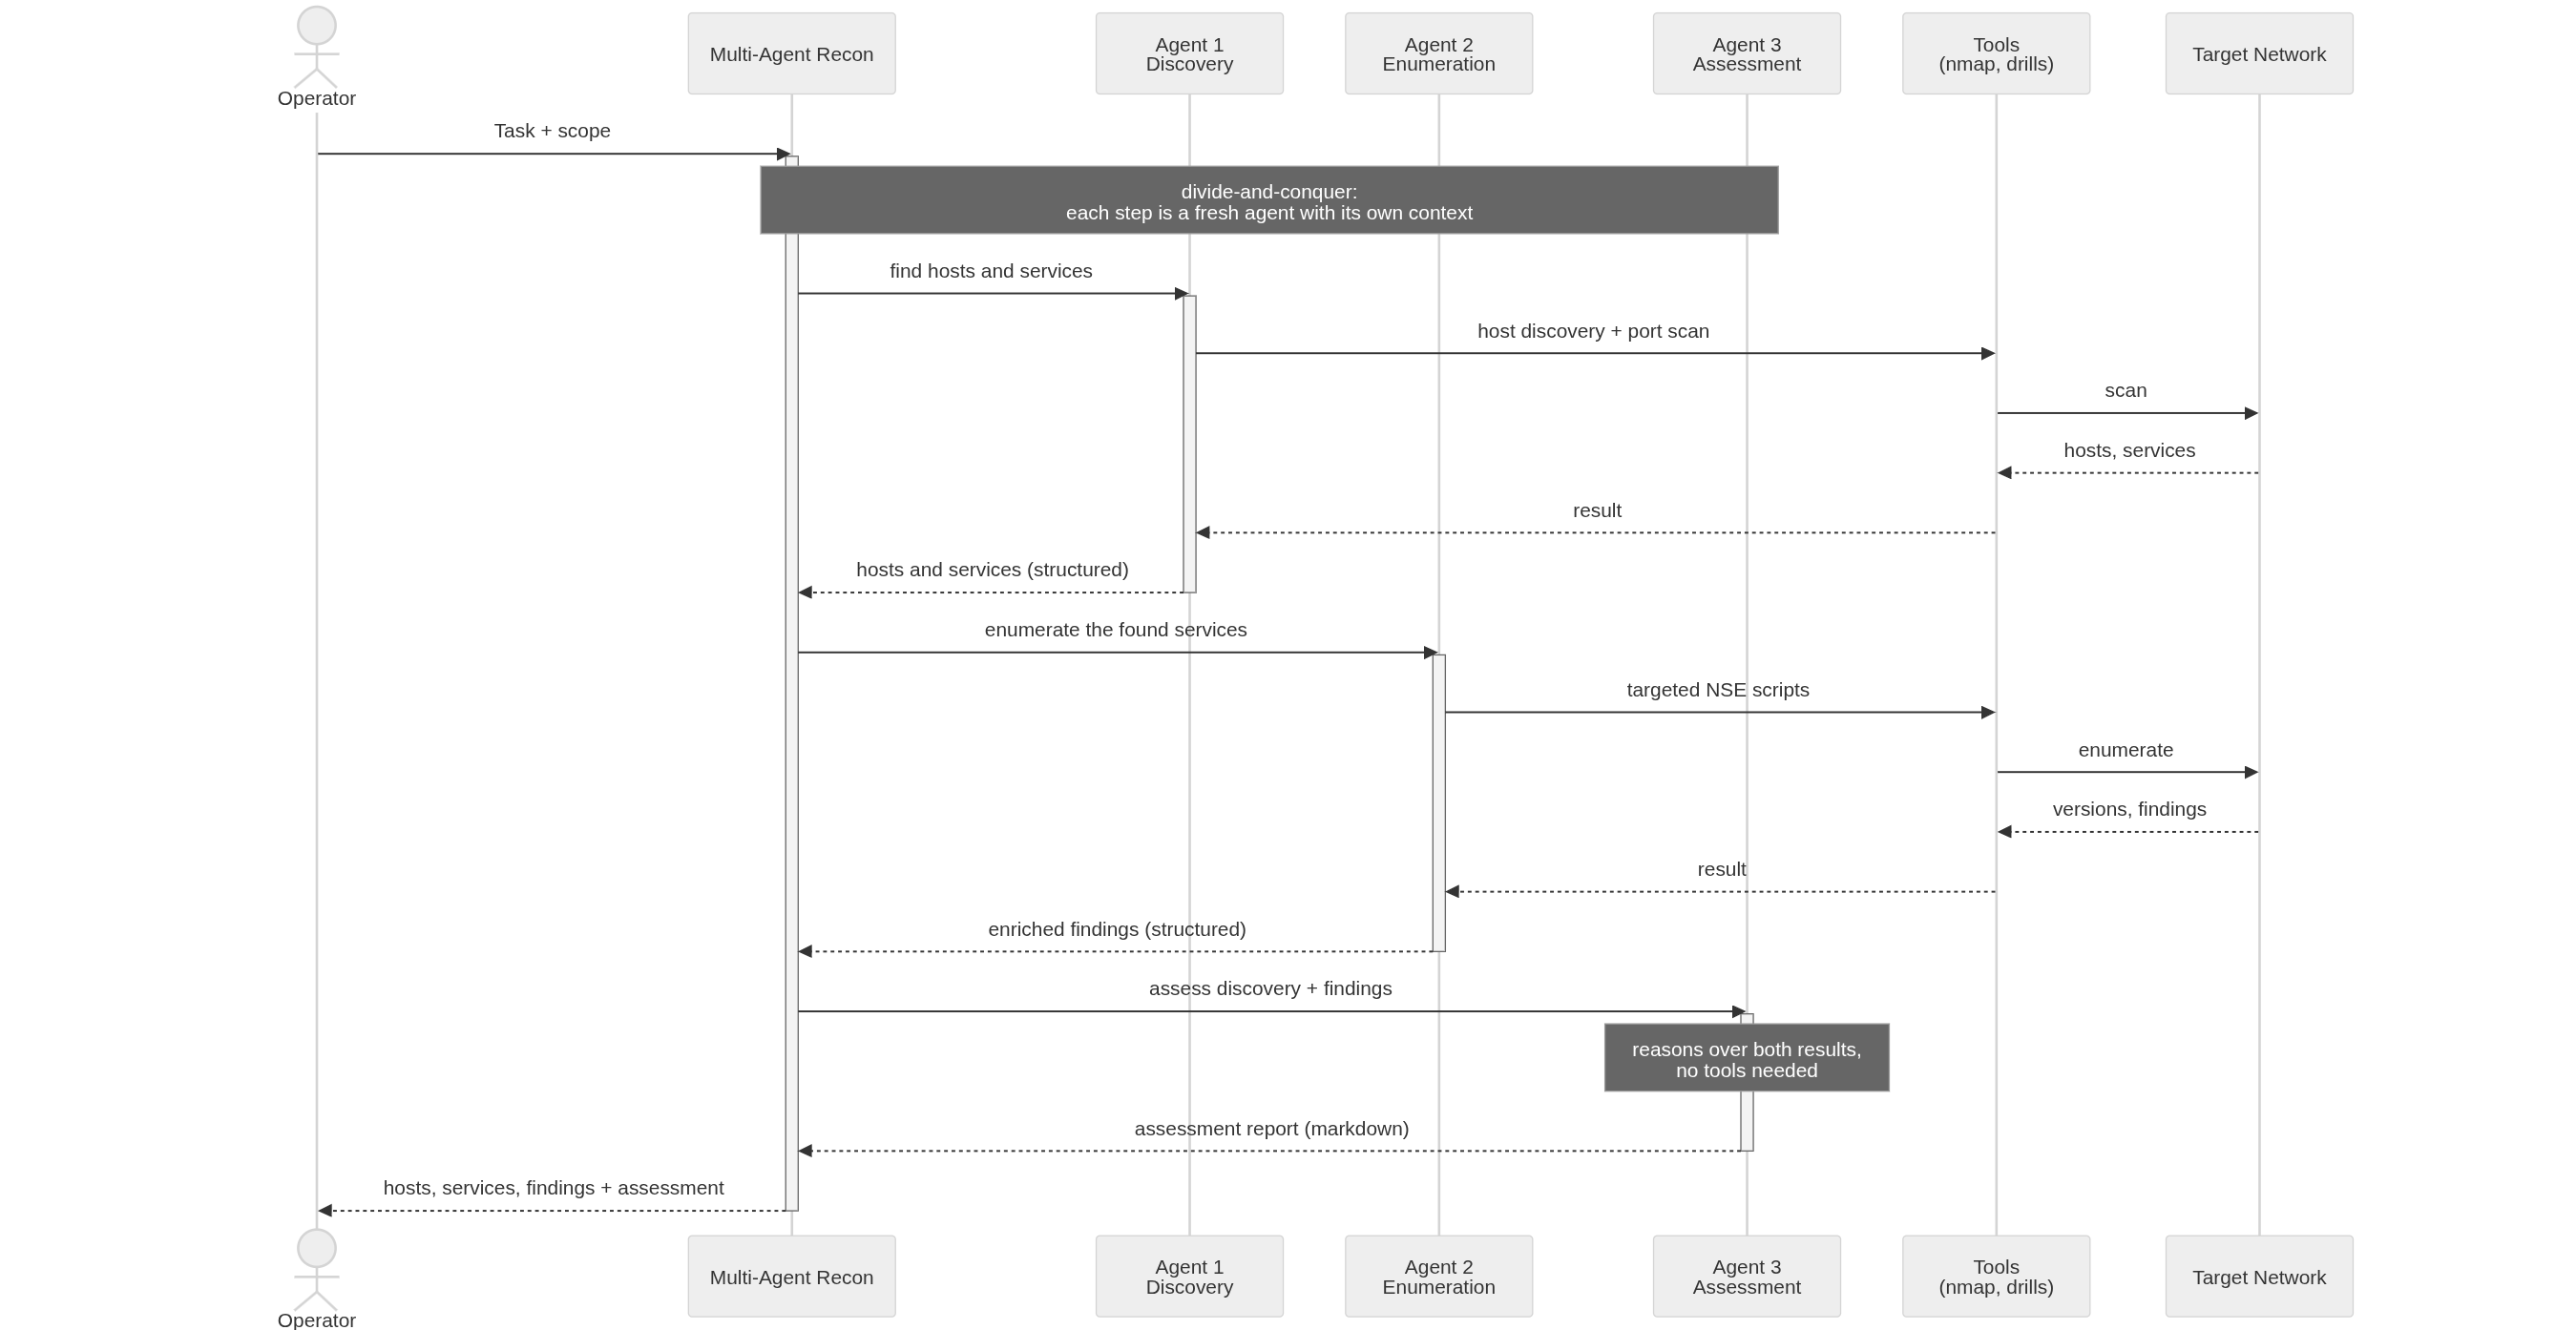
\includegraphics[width=\linewidth,height=0.78\textheight,keepaspectratio]{assets/multi-agent-sequence}
        \label{multi-agent-sequence-diagram}
    \end{figure}
\end{frame}
